\section{Assignment 2: Image Segmentation by $K-$means\ \ Clustering}
\label{sec:assignment2}

In this assignment we use K-means clustering for image segmentation. K-means clustering is a very simple but effective clustering algorithm, but it also comes with some drawbacks. We examine the strengths and weaknesses of this method applied to image segmentation.

\subsection{Problem definition}

Given an image, the goal is to divide it into disjoint regions. These regions should correspond to coherent areas in the image. In  a perfect result, each ``object'' is matched to exactly one region. What an ``object'' is, depends on the application: we might want to separate different colors or textures, or to separate the background from the foreground, or obtain a region for each physical object in the image. In this assignment we examine K-means clustering applied to image segmentation.
 In particular we:
\begin{itemize}[noitemsep]
	\item Implement K-means clustering.
	\item Study the influence of augmenting the color information with spatial information in the form of normalized pixel coordinates.
	\item Study the influence of the number of clusters chosen.
	\item Discuss the advantages and disadvantages of K-means clustering for image segmentation.
\end{itemize}

\subsection{Methodology}

\subsection{Overview}
K-means clustering is an algorithm used to cluster data. It works as follows: assume we have data $x_1,\ldots,x_N \in \mathbb{R}^n$. We first chose K centroids $\mu_k \in \mathbb{R}^n$ randomly. Then we assign each data point $x_i$ to the centroid $\mu_j$ which minimizes the distance between $x_i$ and the centroids $\mu_k$. To record this relation we use an indicator matrix $r(i,j) \in \{0,1\}$, with $r(i,j)=1$ if data point $x_i$ is assigned to centroid $\mu_j$ and $0$ otherwise. We can define an objective function, which the K-means clustering algorithm tries to optimize. For this we define the distortion as
\begin{equation}
	J = \sum_{n=1}^{N} \sum_{k=1}^{K} r(n,k) \left\|x_n-\mu_k\right\|^2.
\end{equation}
This is the sum of squared distances from each data point to its assigned centroid, and we want to minimize it. For this we use the following iterative K-means clustering method:
\begin{enumerate}
\item Initialize the $K$ centroids $\mu_k$ with random values.
\item Assign each data point $x_i$ to its nearest centroid $\mu_j$ and update the indicator matrix
\[
	r(i,j)= \begin{cases}
               1 \text{, if } j = \argmin_k\left\|x_i-\mu_k\right\| \\

             0 \text{ otherwise.}
            \end{cases}
\]
\item Calculate new centroids $\mu_k$ as the mean of all data points assigned to the k-th cluster, i.e. 
\[
	\mu_k = \frac{\sum\limits_{i=1}^N r(i,k) x_i}{\sum\limits_{i=1}^N r(i,k)}
\]
\item Calculate the distortion J with the new assignment and centroids and check for convergence. This is done by checking if the ratio of the old and new $J$ does not change any more, i.e if the ratio lies below a user given threshold. We use the absolute value of 1 minus the ratio, so that the algorithm can also make $J$ a little worse, as this could make the end result better. As long as J does not converge, repeat steps 2 to 4.
\end{enumerate} 

We use two different methods to get data points from pixel values. One is to just take the color values of each pixel, the other is to normalize each coordinate of a pixel to $[0, 1]$ and use the color value and the coordinate of the pixel, resulting in a 5-dimensional space.

To illustrate the results we can color each pixel in the image with the color of the associated centroid. Alternatively we can associate the clusters with mutually distinct colors and colorize the image using these, instead of the value of the centre. This helps to better see the cluster boundaries.

\subsection{Implementation}

You can run the image segmentation with the function \texttt{image\_segmentation(image\_path, K, precision, use\_coordinates, use\_distinct\_colors)}, where \texttt{image\_path} is the path to the image, \texttt{K} is number of clusters, \texttt{precision} is the precision used for the convergence criterion of the distortion, \texttt{use\_coordinates} iis a boolean that says if coordinates should be used or not and \texttt{use\_distinctcolors} is a boolean that if true colors the result with distinct colors or the color of the cluster center otherwise. It returns the segmented image, colored with the chosen option, the cluster centroids and the indicator matrix.
 We will explain some details of the implementation of the next part.

To make use of vectorization and matrix operations we vectorize the image. That means instead of indexing pixels by two indexes we use just one. This has the advantage that the indicator matrix is a two dimensional matrix. Thus we have that $r(i,j)*centroids$, where centroids is the vector of centroids, gives the centroid asspociated with each data point. And if $X$ is the data matrix, i.e $X(i,:)$ is the i-th data point, that $(r(i,j)^T * X$ gives the sum of all data points associated with one cluster.

As mentioned above we use $\vert 1-J_old/J_new\vert < \text{precision}$ as a convergence criterion, where we take absolute values, so that the objective value can also get a worse.

One problem is that calculating the mean of the data of a cluster is not possible if the cluster is empty. This can happen in the assignment stage. To fix this, we choose for each empty cluster a random data point and remove this from its cluster and add it to the empty cluster.

The function distinguishible\_colors waas taken from mathworks.com/matlabcentral/fileexchange and the relevant license is included.
\subsection{Experiments}

We analyzed K-means clustering for image segmentation with the test images \texttt{future.jpg}, \texttt{mm.jpg} and \texttt{simple.PNG}, and made the following experiments: first we clustered each image into 3 and 5 clusters, both with and without the use of coordinates. Then we separately examined the image \texttt{mm.jpg}. We used different K values and varied the use of coordinates. We also ran the algorithm several times on \texttt{simple.PNG} to show the effect of bad initiation.

In the figure \ref{fig:testimages} the test images are shown. The "future.jpg" images shows a drawn image. It contains only a restricted color palette. The test image "mm.jpg" is a photography of a advertisement screen. It has a lot of artifacts in the screen which makes segmentation more difficult. The third test image "simple.PNG" is a artificially generated image. It just contains 2 filled circles on a uniform background. It should be very easy to segment this image.
\begin{figure}[h!]
	
\includegraphics[width=0.38\linewidth]{figures/task2/future.jpg}
	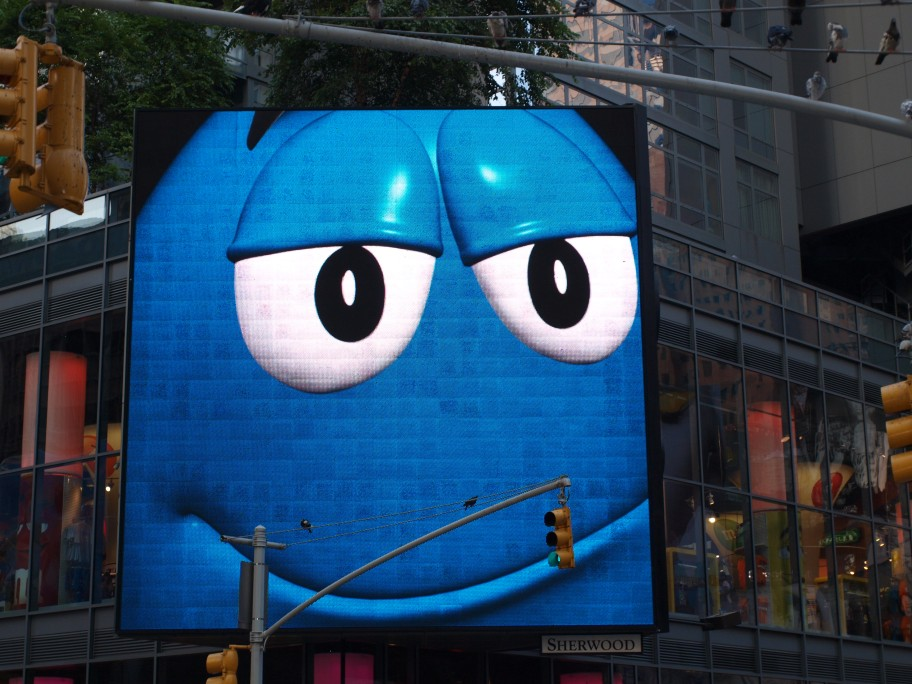
\includegraphics[width=0.398\linewidth]{figures/task2/mm.jpg}
	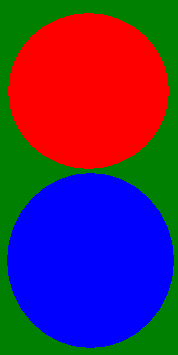
\includegraphics[width=0.15\linewidth]{figures/task2/simple.PNG}
	\caption{The 3 test images. From left to right: future, mm and simple.}
	\label{fig:testimages}
\end{figure}

\subsubsection{Influence of using coordinates}

Figures \ref{fig:future:coords}, \ref{fig:mm:coords} and \ref{fig:simple:coords} illustrate the result of the segmentation by coloring each pixel by the color value of its associated centroid. We show the influence of the usage of coordinates for K=3 and K=5 clusters for each test image.
\begin{figure}[h!]
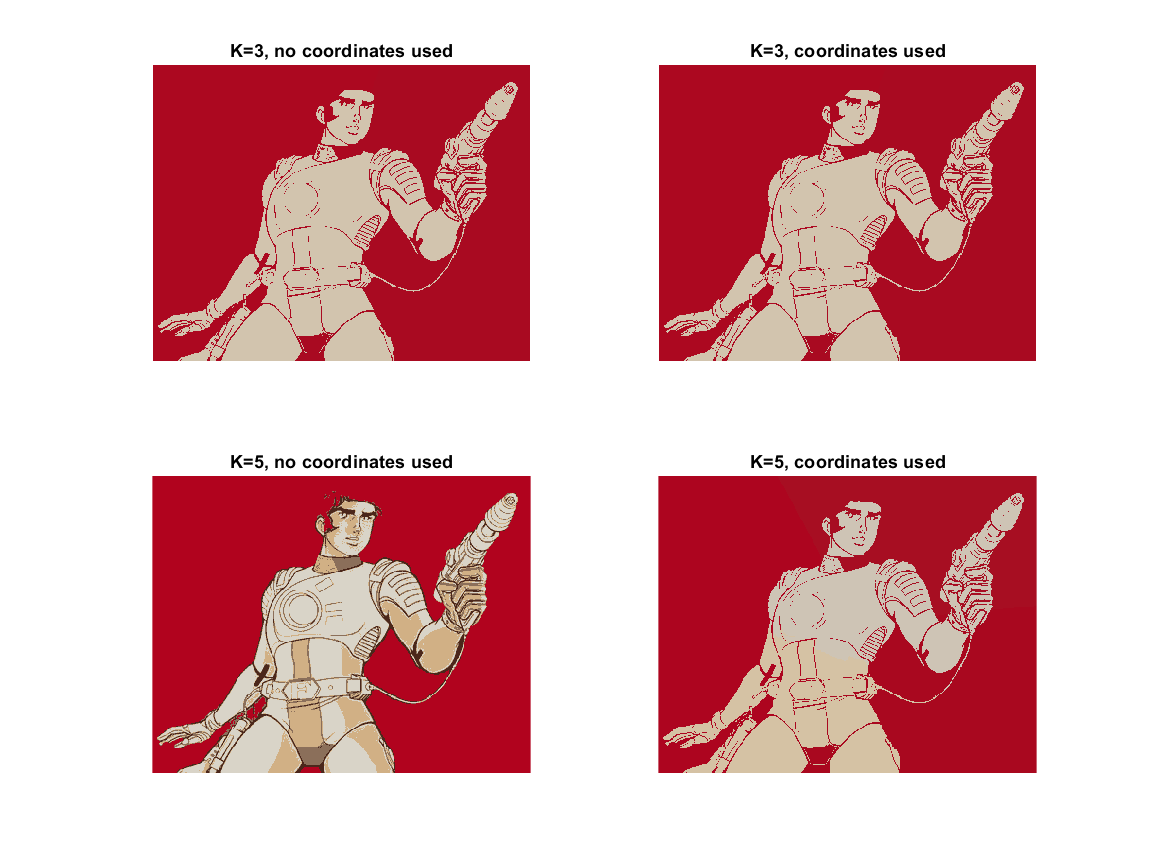
\includegraphics[width = 0.9\linewidth]{figures/task2/future_coordinates.png}
\caption{Coordinate experiment for \texttt{future.jpg}}
\label{fig:future:coords}
\end{figure}

For the "future.jpg" image we can see that the segmentation without using coordinates produces a pleasing result. It can separate the different colors very accurately. This is the case as the image contains only a limited number of colors, and all colors in a coherent region have the same color. For the clustering with coordinates it appears that the algorithm found less clusters than K. This is the case as the background gets segmented into multiple regions. This happens, because the pixels on the right and on the left have on one hand the same color, but are spatially far apart, so it makes sense to split the background in a left region and right region. For $K=5$ the image gets split into 3 background region a top part of person region and a bottom part of person region. We can see that not only the color is important, but also the spacial relation. We can already see here, that using the colors of the cluster center makes the inspection of the result hard, as several cluster, in particular for the case which uses coordinates, can have the same or very similar colors.
\begin{figure}
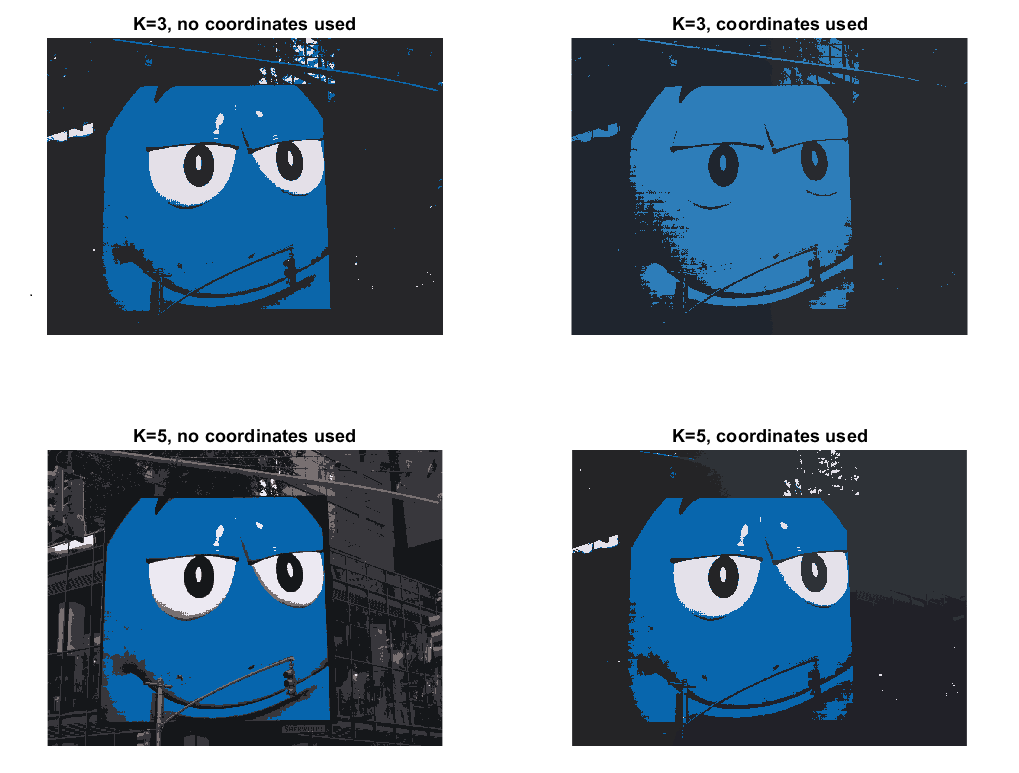
\includegraphics[width = 0.9\linewidth]{figures/task2/mm_coordinates.png}
\caption{Coordinate experiment for \texttt{mm.jpg}}
\label{fig:mm:coords}
\end{figure}


\begin{figure}[h]
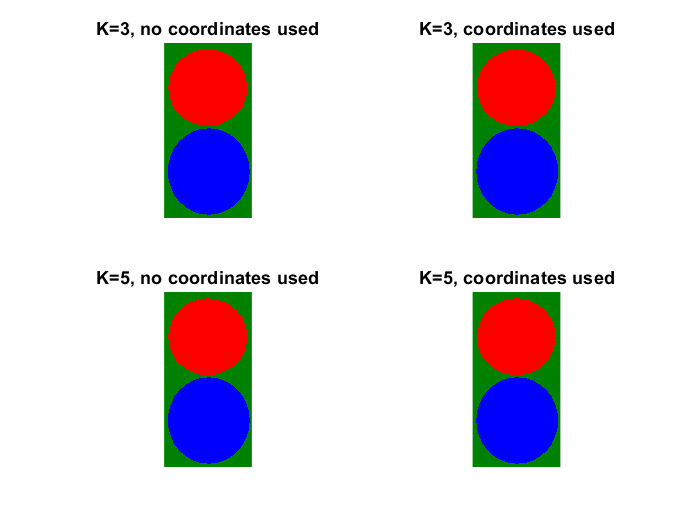
\includegraphics[width = 0.9\linewidth]{figures/task2/simple_coordinates.png}
\caption{Coordinate experiment for \texttt{simple.PNG}}
\label{fig:simple:coords}
\end{figure}

